\documentclass{article}
\usepackage[utf8]{inputenc}
\usepackage{mathtools}
\usepackage{amssymb}
\usepackage{graphicx}
\usepackage{listings}
\usepackage{float}
\usepackage{gensymb}
\usepackage{amsthm}
\usepackage{longtable}
\usepackage{adjustbox}
\usepackage{physics}
\usepackage[makeroom]{cancel}

\theoremstyle{definition}
\newtheorem{definition}{Definition}
\newtheorem{proposition}{Proposition}

\title{Statistical Field Theory}
\author{quinten tupker}
\date{October 9 2020 - \today}

\begin{document}

\maketitle

\section*{Introduction}

These notes are based on the course lectured by Dr Christopher E Thomas in
Michaelmas 2020. Due to the measures taken in the UK to limit the spread of
Covid-19, these lectures were delivered online. These are not meant to be an
accurate representation of what was lectures. They solely represent a mix of
what I thought was the most important part of the course, mixed in with many
(many) personal remarks, comments and digressions... Of course, any
corrections/comments are appreciated.

Statistical Field Theory is an extension of statistical physics. It assumes one
is familiar with statistical physics, and in particular, focuses on the study on
phase transitions. This course in particular follows David Tong's notes quite
closely.

\section{From Spin to Fields}

So why do we consider fields? Here we look at a model that shows the origin of
this connection.

\subsection{The Ising model}

The Ising model studies a lattice where each point on the lattice is assigned a
spin $S_i = \pm$. Consequently, the energy of the lattice is

$$ E = -B \sum_i S_i - J \sum_{<i, j>} S_i S_j $$

where $B$ is the external magnetic field strength, $J$ is the strength of
neighbour-neighbour interactions and $<i, j>$ is any nearest neighbour pair.
When $J > 0$, states tend to align (ferromagnetic behaviour) whereas if $J < 0$
states will prefer not to align (anti-ferromagnetic behaviour). We will focus on
the $J > 0$ case. But of course, due to heat there some statistical randomness,
and we want to include that. As such, we consider the canonical ensemble with
$\mathbb{P} (S_i) = e^{-\beta E(S_i)} / Z$ where $Z$ is the partition function,
$\beta = 1 / T$, and the Boltzmann constant $k_B = 1$. As ever in statistical
physics, we can derive everything from the partition function. Particularly
important in our case is the Free Energy, $F = \langle E \rangle - TS = -T \ln
(Z)$, and $dF = -S dT - p dV - M dB$ (so we can find S, p and M from F as well).

In statistical physics, we are particularly interested in the equilibrium state
(which occurs at the minimum of the free energy when temperature is constant),
and since we are looking at a magnetic system, we are particularly interested in
the equilibrium magnetisation. This can be calculated as

$$ m = \frac{1}{N} \sum_i \langle S_i \rangle = \frac{1}{N \beta} \partial_B
\ln(Z) $$

Now all that remains is to calculate $Z$ to find $m$. Unfortunately, in
dimension 3 or greater this is impossible (how impossible?), and it is still
hard in lower dimension. Consequently we take a different approach using the
so-called ``effective free energy'', which is defined such that

$$ \sum_m \sum_{\{S_i\} | m} e^{-\beta E[S_i]} = \sum_m e^{-\beta F(m)} $$

where $F(m)$ is the effective free energy. Since we can assume $N$ is large
(around $10^{23}$), we can then write18

$$ Z = N / 2 \int_{-1}^1 dm \, e^{-\beta F(m)}  = N / 2 \int_{-1}^1 dm \,
e^{-\beta N f(m)}$$

where $f(m) = F(m) / N$. From here, we can calculate the equilibrium field by
considering that since $N$ is large, the value contributing the most to the
integral is where $\partial_m f = 0$, and this is how the equilibrium $m$ is
calculated. This approach is called the \textbf{steepest descent approximation},
and we find here that $F_{\text{thermodynamic}} \approx F(m_{\text{min}})$.

This is all very well and nice, but the issue is that we still don't know how to
calculate $F(m)$, and it turns out that this is about as hard as calculating
$Z$. As such, we use the \textbf{mean field approximation}

$$ E \approx -B \sum_i m - J \sum_{<i, j>} m^2 = -BNm - \frac{1}{2} N J q m^2 $$

where $q = 2 \text{dim(space)}$ for a cubic latice in a space dimension dim.
Now,

$$ e^{-\beta N f(m)} = \sum e^{-\beta E(S_i) \approx \Omega(m) e^{-\beta
    E(m)}} $$

so in order to find $f(m)$ we need to know $\Omega(m)$ which is the number of
ways for a given energy state to occur, but since $m$ depends only on the number
of positive and negative spins states, $N_\uparrow, N_\downarrow$, and in
particular $N = N_\uparrow + N_\downarrow$ we see the number of total states is

$$ \ln(\Omega) = \ln \binom{N}{N_\uparrow} \approx N (\ln(2) - \frac{1}{2}(1 +
m) \ln(1 + m) - \frac{1}{2} (1 - m) \ln(1 - m)) $$

by Stirling's approximation. Consequently we find that

$$ f(m) \approx -Bm - \frac{1}{2} J q m^2 - \frac{1}{\beta} (\ln(2) -
\frac{1}{2} (1 + m) \ln(1 + m) - \frac{1}{2} (1 - m) \ln(1 - m)). $$

From here  by taking $\partial_m f = 0$, we find

$$ \beta(B + Jqm) = \frac{1}{2} \ln \left( \frac{1 + m}{1 - m} \right) $$

or equivalently

$$ m = \tanh(\beta (B + Jqm)). $$

From here, we can solve implicitly, but there is another approach we can take,
which is the way we will go about this. Just as a side note, we can see the
reason this is called the mean field approximation here as well: it is as if $m$
just shifts to external field to $B_{\text{eff}} = B + Jqm$. [End of lecture 1.]

\subsection{Landau Theory of Phase Transitions}

The remarkable part about the Ising model described above is not its
correctness. In fact, it is often incorrect, but rather its universality. It can
be applied in a wide variety of situations. As such, Landau tried to develop a
more general theory of phase transitions. Here we work through an extended
example to examine the general features of these. In particular, we study the
behaviour of the equilibrium $m_{\text{min}}$ when various quantities are varied.

From before, we can approximate $f$ for small $m$ as

$$ f(m) \approx \cancel{-\frac{1}{\beta} \ln(2)} - B m + \frac{1}{2} (\frac{1}{\beta} -
Jq) m^2 + \frac{1}{12\beta} m^4 + \dots $$

where we ignore the constant term since it does not affect anything. We start
with the $B = 0$ case where we find that

$$ f(m) = \frac{1}{2} (T - T_c) m^2 + \frac{1}{12} T^4 m^4  $$

where we define the \textbf{critical temperature} to be $Tc = Jq$. Then we get
the following scenarios.

\begin{figure}[H]
  \centering
  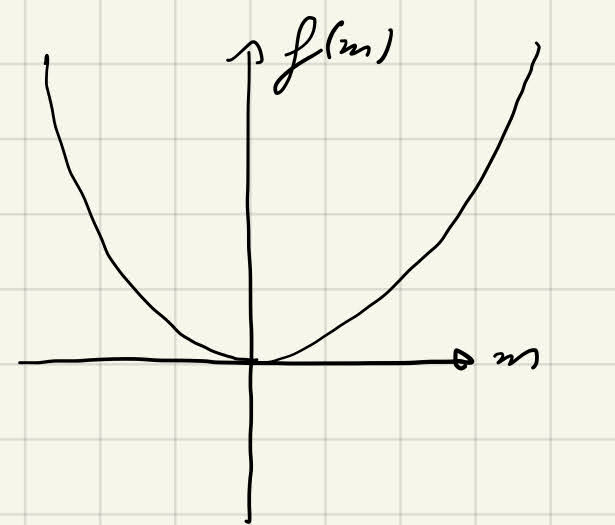
\includegraphics[width=5cm]{res/SFT/f_vs_m_high_T_B0}
  \caption{$T > T_c$}
  \label{figure: f_vs_m_high_T_B0}
\end{figure}

\begin{figure}[H]
  \centering
  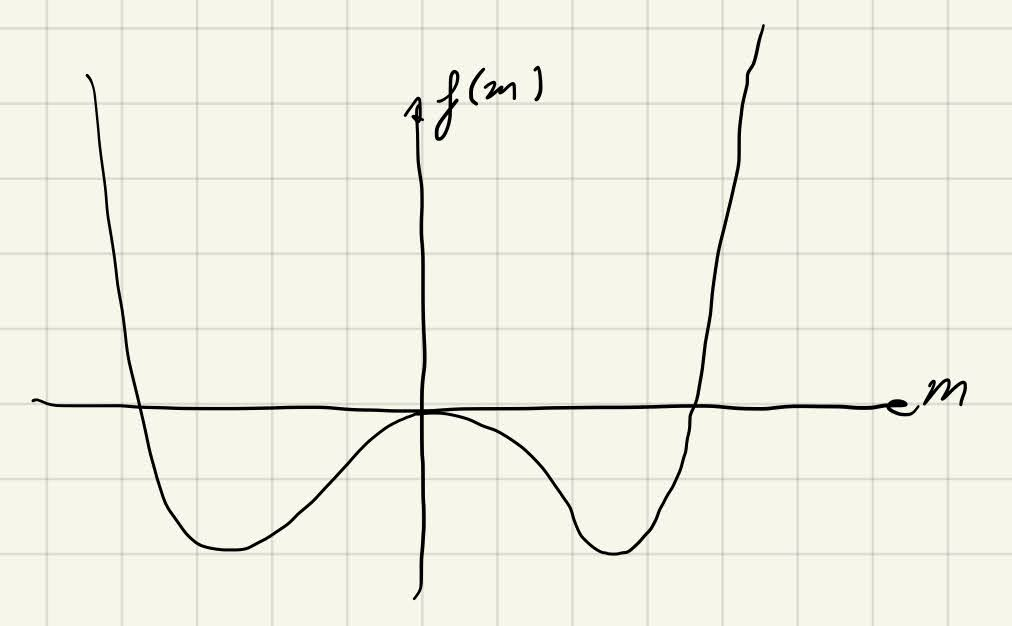
\includegraphics[width=5cm]{res/SFT/f_vs_m_low_T_B0}
  \caption{$T < T_c$}
  \label{figure: f_vs_m_low_T_B0}
\end{figure}

\begin{figure}[H]
  \centering
  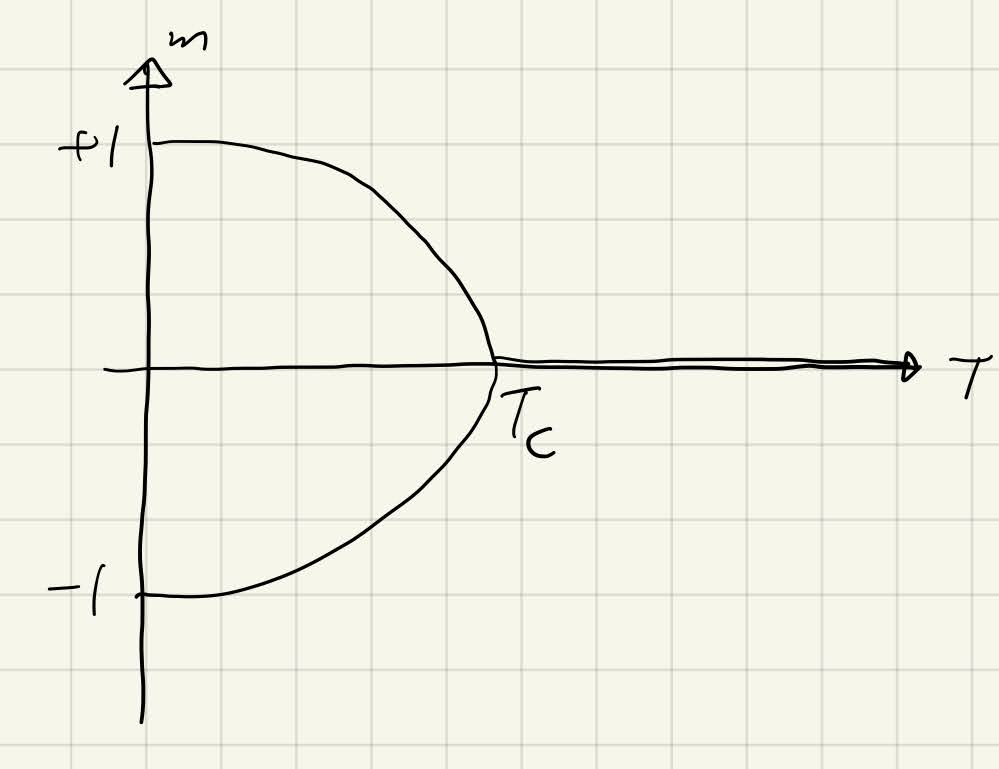
\includegraphics[width=5cm]{res/SFT/m_vs_T_B0}
  \caption{$m_{\text{min}}(T)$ for $B = 0$}
  \label{figure: m_vs_T_B0}
\end{figure}

The middle graph is meant to be symmetric, and we see here that $m_{\text{min}}$
can take two different values

$$ m_{\text{min}} = \pm m_0 = \pm \sqrt{\frac{3(T_c - T}{T}} $$

Now some definitions apply here. This is a \textbf{second order} or
\textbf{continuous} phase transition since $m$ is continuous in the quantity
being varied. $m = 0$ is called the \textbf{disordered phase}, and $m \neq 0$ is
called an \textbf{ordered phase}. \textbf{Spontaneous symmetry breaking} is what
we call the loss of symmetry in $m$ when $T$ decreases below $T_0$ (since $m$ is
forced to choose a positive or negative value). Finally, these terms all extend
to arbitrary \textbf{order parameter} $m$. We finally compute

$$ f(m_{\text{min}}) =
\begin{cases}
  0 & T > T_c \\
  -\frac{3}{4} \frac{(T_c - T)^2}{T} & T < T_c
\end{cases} $$

We can also look at the heat capacity here, and how that various with
temperature. Heat capacity may be defined as

$$ C = \partial_T \langle E \rangle = \beta^2 \partial_\beta^2 \ln(Z) $$

since recall that $\langle E \rangle = -\partial_\beta \ln(Z)$. Using $Z \approx
-\beta N f(m_{\text{min}})$ we find $c = C / N$ has

$$ c =
\begin{cases}
  0 & T \to T_c^+ \\
  3/2 & T \to T_c^-
\end{cases}
$$

so $c$ is a first order phase transition - ie. discontinuous.

The above scenario considered $B \neq 0$, but when $B = 0$ we get a different
situation. In particular, we do not get spontaneous symmetry breaking since the
system is no longer symmetric. In this case, the above graphs are skewed to the
right or the left unevenly leaving global minimum (the ``true'' minimum) and a
so-called \textbf{metastable} state.

Finally, we can observe another discontinuous phase transition when we study
$m_{\text{min}}$ as a function of $B$ at low $T$ ($T < T_c$). Since we're below
the critical temperature, the global minimum does not smoothly slide through 0,
but instead abruptly shifts from negative to postive (or the other way around)
giving a 1st order phase transition. Incidentally, I find this a bit odd, since
this really only makes sense in the 1D case, but as we will see later Mean Field
Theory (MFT) does not work in 1D. But in higher dimensions, $m$ is a vector and
instead of getting two local minima as above, we get a tilted (for $B \neq 0$)
circular valley where $f(m)$ is low. In this case, no phase transition occurs,
since the minimum just smoothly moves around this circular valley as $B$ is
varied...

\begin{figure}[H]
  \centering
  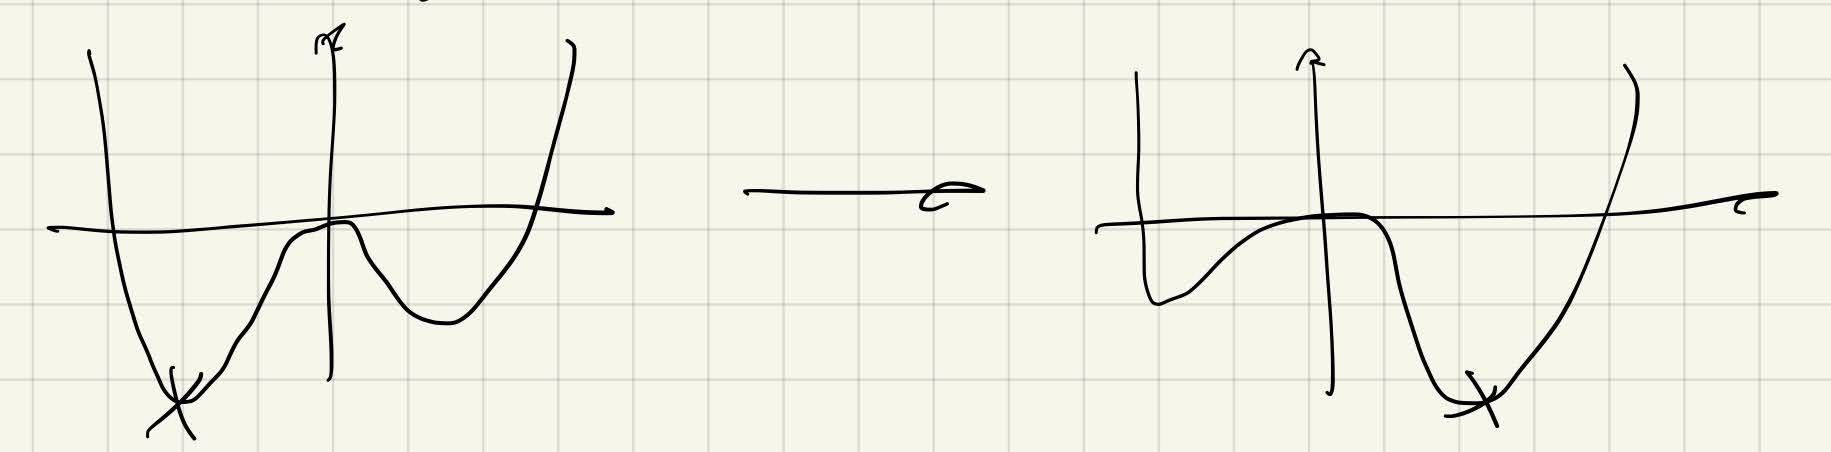
\includegraphics[width=10cm]{res/SFT/m_min_vs_B}
  \caption{$m_{\text{min}}$ vs $B$}
  \label{figure: m_min_vs_B}
\end{figure}

\begin{figure}[H]
  \centering
  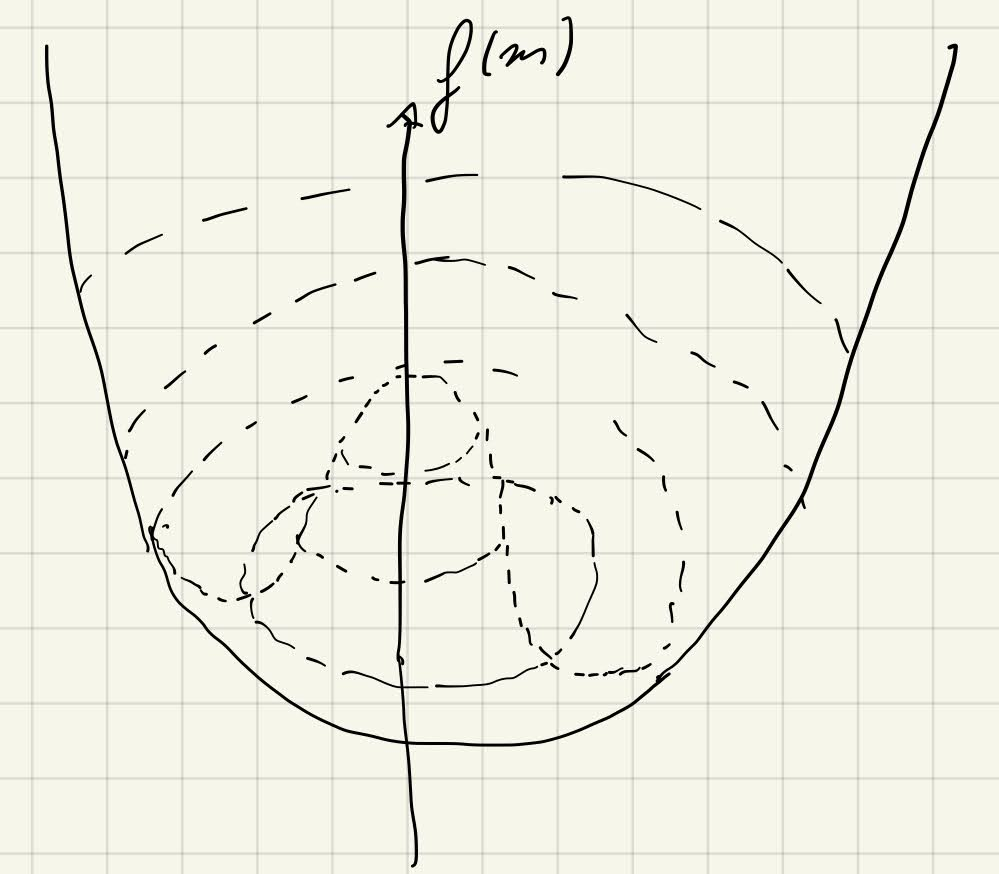
\includegraphics[width=5cm]{res/SFT/f_vs_m_2d}
  \caption{$f(m)$ vs $m$ in 2D}
  \label{figure: f_vs_m_2d}
\end{figure}

Anyways, some other asymptotic behaviour includes that when $T \approx T_c$, we
get

$$ f(m) \approx -Bm + \frac{1}{12} T_c m^4 $$

leaving

$$ m \sim B^{1/3} $$

If we define magnetic susceptibility (the \textbf{response function} in this
context) to be $\chi = \partial_B m|_T$ we see that for $T > T_c$ we have

$$ f(m) \approx -Bm + \frac{1}{2} (T - T_c) m^2 + \dots $$

so

$$ m \approx \frac{B}{T - T_c} $$

so

$$ \chi \sim \frac{1}{T - T_c} $$

and for $T < T_c$

$$ \chi \sim \frac{1}{|T - T_c|} $$

\subsection{The Validity of MFT}

The purpose of all these calculations at the end of the last section is to find
some important set of numbers that we can use to check our theory with in the
real world. In particular, what we looked for were the \textbf{critical
  exponents}, which are

\begin{align*}
  m &\sim (T_c - T)^\beta & \beta &= 1/2 & T &< T_c \\
  c &\sim c_\pm |T - T_c|^{-\alpha} & \alpha &= 0 && \\
  \chi &\sim |T - T_c|^{-\gamma} & \gamma &= 1 && \\
  m &\sim B^{1/\delta} & \delta &= 3 &&
\end{align*}

in our worked example. Now for results, we find that in general, MFT fails
entirely below a certain \textbf{lower critical dimension}, $d_i$ and works correctly
above a certain \textbf{upper critical dimension}, $d_u$. In between it is structurally
accurate (can detect the right phase transitions) but inaccurate (finds the
wrong critical exponents). The Ising fails for dimension 1, gets the right
structure for dimensions 2 and 3, and works for dimension 4 and above. It is, as
expected, closer to the correct value for dimension 3 than for 2, but still can
be quite off.

Nevertheless, as mentioned earlier, the power of the MFT is not in its
correctness, but in its universality. Also, often structure is more important.
After all, if you can predict a phenomenon will happen, you can then carry out
an experiment to measure it more accurately. On the other hand, it is far harder
to use experiment to search for interesting phenomenon without knowing where to
look. So it is still quite powerful. Also, the fact that critical
exponents exist, and that critical points exist is a powerful bit of
universality that MFT gives.

To illustrate its universality, we can consider liquid-gas transitions. Here,
van der Waals analysis is completely off in its critical exponents, although it
does predict the correct type of phenomenon. However in three dimensions, the
Ising model agrees well. How do we implement the Ising model for a gas. Although
it's not at all obvious it will work, the implementation is actually quite
natural. Assume that a space consists of a lattice, and that every lattice is
assigned a value of 1 or 0 based on whether or not it is occupied by a particle.
Also assume that any point on the lattice can be occupied by no more than 1
particle at a time. Then we get

$$ E = -4J \sum_{<i j>} n_i n_j - \mu \sum n_i $$

We can proceed from there as usual. [End of lecture 2]

\subsection{Landau-Ginzburg Theory}

We aim to improve on Landau theory, and somehow the obvious generalisation is to
allow $m$ to vary through space as $m(x)$, but doing so in a way that it is
analytic, so that the calculations involved still stay relatively simple...

Concretely, that means assuming we have a large number of sites $N$, but that
these sites are all grouped into clusters of $N'$ sites, which is still a large
number, but significantly smaller than $N$. Then we define for each cluster, a
centre $x$, and we assign $m(x)$ the value of the average magnetisation of this
cluster. However, since $1 << N' << N$, everything is still analytic, etc. Or so
we assume.

Consequently we can calculate the partition function in much the same way with
the same effective free energy, except now the effective free energy is a
functional instead of a function:

$$ Z = \sum_{m(x)} e^{-\beta F[m(x)]} $$

This can be written as a functional integral (otherwise known as a path integral)

$$ Z = \int Dm[x] e^{-\beta F[m(x)]} $$

and now instead of probabilities we get probabilty density

$$ p(m(x)) = \frac{e^{-\beta F[m(x)]}}{Z}. $$

Now, we have a number of conditions that we require this effective free energy
to satisfy:

\begin{itemize}
\item locality: basically, it takes the form
  $$ F[m(x)] = \int d^dx f[m(x)] $$
  where $f$ depends on $m, \nabla m, \nabla^2 m, \dots$
\item $\mathbb{Z}_2$ symmetry when $B = 0$ under $m \mapsto -m$
\item Analyticity - we assume it has a Taylor expansion
\item we are only interested in $m$ that are slowly varying in space
\end{itemize}

Now, focusing on the $B = 0$ case we see that the effective free energy must
take the form

$$ F[m(x)] = \int dx (\frac{1}{2} \alpha_2(T) m^2 + \frac{1}{4} \alpha_4(T) +
\frac{1}{2} \gamma(T) (\nabla m)^2) $$

where the odd terms are eliminated due to symmetry (of course, when $B \neq 0$
we can add in these odd terms again).

Unfortunately it is hard to find an general way to calculate $\alpha_2,
\alpha_4, \gamma$. but we can say that $\alpha_4, \gamma > 0$ and $\alpha_2$
changes sign at $T_c$/ In particular, in MFT,

$$ \alpha_2 \sim (T - T_c), \alpha_4 \sim \frac{1}{3} T. $$

Just as in plain Landau theory, we use the saddle point approximation that $Z =
\int dm(x) e^{-\beta F(m(x))}$ is focused on the saddle point of $F$, but this
time to find it we need to use the Euler-Lagrange approach, yielding the
equation for the equilibrium:

$$ \gamma \nabla^2 m = \alpha_2m + \alpha_4 m^3 $$

How well does this theory work? We can check that if we assume $m$ is constant,
then we get back to Landau theory, so we know that at the very least, this
theory cannot be worse than Landau theory. As our first development we then look
at the notion of domain walls, and see whether or not those can be of any help.
In particular, we want to see what a solution to the following looks like in the
one dimensional case:

$$ \partial_x^2 m = \alpha_2 m + \alpha_4 m $$ 

where $m = \pm m_0$ as $x \to \pm \infty$. The solution works out to $m = m_0
\tanh(\frac{x - x_0}{W})$ where the width, $W = \sqrt{-\gamma / \alpha_2}$.

This models how the system changes state half-way, and since these don't occur
in ordinary Landau theory. As such, to compare the two it would be helpful to
see what the free energy cost of having a domain wall is. We may calculate this
as

\begin{align*}
  F_W
  &\sim L^{d - 1} \int dx \gamma(\partial_x)^2 \\
  &\sim L^{d - 1} \gamma m_0^2 / W \\
  &= L^{d - 1} \sqrt{-\gamma \alpha_2^3 / \alpha_4^2}
\end{align*}

where $L$ is the ``length'' of the system. Now curiously, this allows us to see
why Landau fails in 1 dimension, but not (as much) in 2 dimensions.

Consider a 1 dimensional space length $L$, starting in state $m_0$ and ending in
some other state, for $T < T_c$, meaning that $\alpha_2 < 0$. We then see that

$$ \mathbb{P}(\text{wall at } x = x_0) = \frac{e^{-\beta F_W}}{Z} $$

$$ \mathbb{P}(\text{wall somewhere}) \sim \frac{L}{W} \frac{e^{-\beta
    F_W}}{Z} $$

meaning that

$$ \mathbb{P}(n \text{ walls}) = e^{-n\beta F_W} / Z \int_0^L dx_1 \int_{x_1}^L
dx_2 \dots \int_{x_{n - 1}}^L dx_n = \frac{1}{Z n!} \left( \frac{L e^{-\beta
      F_W}}{W} \right)^n. $$

Consequently we can calculate the probabilities of how the final state of the
rod ends up:

$$ \mathbb{P}(m \to m_0) = \frac{1}{Z} \cosh \left( \frac{Le^{-\beta F_W}}{W}
\right) $$

$$ \mathbb{P}(m \to -m_0) = \frac{1}{Z} \sinh \left( \frac{Le^{-\beta F_W}}{W}
\right) $$

Now as $L \to \infty$, we see that these probabilities stay about the same,
meaning that the state of the rad stays more or less random. Why does this
argument fail in two dimensions? Well, the calculation does change a bit since
we're in two dimensions, but we also have the fact that $F_W$ may depend on $L$
in this scenario, meaning that in effect, the probabilities above instead
converge to 0 and 1, meaning that a phase transition does indeed occur. [End of
lecture 4]

\end{document}